\documentclass[10pt]{exam}

\usepackage{amssymb, amsmath, amsthm, mathrsfs, multicol, graphicx}
\usepackage{tikz}

 \def\d{\displaystyle}
\def\?{\reflectbox{?}}
\def\b#1{\mathbf{#1}}
\def\f#1{\mathfrak #1}
\def\c#1{\mathcal #1}
\def\s#1{\mathscr #1}
\def\r#1{\mathrm{#1}}
\def\N{\mathbb N}
\def\Z{\mathbb Z}
\def\Q{\mathbb Q}
\def\R{\mathbb R}
\def\C{\mathbb C}
\def\F{\mathbb F}
\def\A{\mathbb A}
\def\X{\mathbb X}
\def\E{\mathbb E}
\def\O{\mathbb O}
\def\U{\mathcal U}
\def\pow{\mathcal P}
\def\inv{^{-1}}
\def\nrml{\triangleleft}
\def\st{:}
\def\~{\widetilde}
\def\rem{\mathcal R}
\def\sigalg{$\sigma$-algebra }
\def\Gal{\mbox{Gal}}
\def\iff{\leftrightarrow}
\def\Iff{\Leftrightarrow}
\def\land{\wedge}
\def\And{\bigwedge}
\def\AAnd{\d\bigwedge\mkern-18mu\bigwedge}
\def\Vee{\bigvee}
\def\VVee{\d\Vee\mkern-18mu\Vee}
\def\imp{\rightarrow}
\def\Imp{\Rightarrow}
\def\Fi{\Leftarrow}

%\def\={\equiv}
\def\var{\mbox{var}}
\def\mod{\mbox{Mod}}
\def\Th{\mbox{Th}}
\def\sat{\mbox{Sat}}
\def\con{\mbox{Con}}
\def\bmodels{=\joinrel\mathrel|}
\def\iffmodels{\bmodels\models}
\def\dbland{\bigwedge \!\!\bigwedge}
\def\dom{\mbox{dom}}
\def\rng{\mbox{range}}
\DeclareMathOperator{\wgt}{wgt}


\def\bar{\overline}


\newcommand{\vtx}[2]{node[fill,circle,inner sep=0pt, minimum size=4pt,label=#1:#2]{}}
\newcommand{\va}[1]{\vtx{above}{#1}}
\newcommand{\vb}[1]{\vtx{below}{#1}}
\newcommand{\vr}[1]{\vtx{right}{#1}}
\newcommand{\vl}[1]{\vtx{left}{#1}}
\renewcommand{\v}{\vtx{above}{}}

\def\circleA{(-.5,0) circle (1)}
\def\circleAlabel{(-1.5,.6) node[above]{$A$}}
\def\circleB{(.5,0) circle (1)}
\def\circleBlabel{(1.5,.6) node[above]{$B$}}
\def\circleC{(0,-1) circle (1)}
\def\circleClabel{(.5,-2) node[right]{$C$}}
\def\twosetbox{(-2,-1.4) rectangle (2,1.4)}
\def\threesetbox{(-2.5,-2.4) rectangle (2.5,1.4)}
\newcommand{\twoline}[2]{\begin{pmatrix}#1 \\ #2 \end{pmatrix}}


\def\circleA{(-.5,0) circle (1)}
\def\circleAlabel{(-1.5,.6) node[above]{$A$}}
\def\circleB{(.5,0) circle (1)}
\def\circleBlabel{(1.5,.6) node[above]{$B$}}
\def\circleC{(0,-1) circle (1)}
\def\circleClabel{(.5,-2) node[right]{$C$}}
\def\twosetbox{(-2,-1.5) rectangle (2,1.5)}
\def\threesetbox{(-2,-2.5) rectangle (2,1.5)}

\newcommand{\onedot}{
  +(.5,.5) \v
}
\newcommand{\twodots}{
  +(.25,.25) \v +(.75,.75) \v
}
\newcommand{\threedots}{
+(.25,.25) \v +(.5, .5) \v +(.75,.75) \v
}
\newcommand{\fourdots}{
  +(.25,.25) \v +(.25,.75) \v +(.75,.25) \v +(.75,.75) \v
}
\newcommand{\fivedots}{
  +(.5,.5) \v +(.25,.25) \v +(.25,.75) \v +(.75,.25) \v +(.75,.75) \v
}
\newcommand{\sixdots}{
  +(.25,.5) \v +(.75,.5) \v +(.25,.25) \v +(.25,.75) \v +(.75,.25) \v +(.75,.75) \v
}
\newcommand{\dominoborder}{
  \draw[thick, rounded corners] (0,0) rectangle (1,2);
  \draw[thin] (0,1) -- (1,1);
}

%\pointname{pts}
\pointsinmargin
\marginpointname{pts}
\marginbonuspointname{pts-bns}
\addpoints
\pagestyle{head}
% \printanswers

\firstpageheader{Math 228}{\textbf{Homework 2}}{Due: September 7}


\begin{document}
\noindent \textbf{Instructions}: Complete the homework problems below on {\em separate} sheets of paper (and not all jammed up between the questions).  This is to be turned in and graded, so make sure your work is neat and easy to read -- there is nothing wrong with using a \underline{separate sheet} of paper for each problem. Your work will be graded on correctness as well as the clarity of your explanations.  You may work with other students in this class on solving the problems, but your write-ups should be completed individually.  You are not permitted to search for solutions online or in other textbooks.

\begin{questions}


\question[6] On the table rest 8 dominoes, as shown below.  If you were to line them up in a single row, so that any two sides touching had matching numbers, what would the sum of the two end numbers be?

\centerline{
		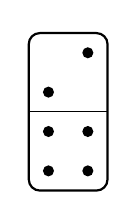
\begin{tikzpicture}
			\dominoborder
			\draw (0,0) \fourdots (0,1) \twodots;;
		\end{tikzpicture}
		\hspace{1em}
		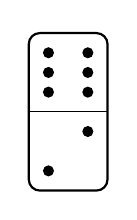
\begin{tikzpicture}
			\dominoborder
			\draw (0,0) \twodots (0,1) \sixdots;
		\end{tikzpicture}
		\hspace{1em}
	 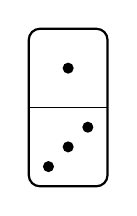
\begin{tikzpicture}
		\dominoborder
		 \draw (0,0) \threedots (0,1) \onedot;
	 \end{tikzpicture}
	 \hspace{1em}
	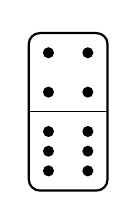
\begin{tikzpicture}
	 \dominoborder
		\draw (0,0) \sixdots (0,1) \fourdots;
	\end{tikzpicture}
	\hspace{1em}
 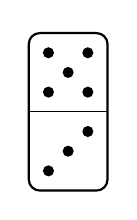
\begin{tikzpicture}
	\dominoborder
	 \draw (0,0) \threedots (0,1) \fivedots;
 \end{tikzpicture}
 \hspace{1em}
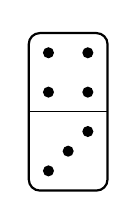
\begin{tikzpicture}
 \dominoborder
	\draw (0,0) \threedots (0,1) \fourdots;
\end{tikzpicture}
\hspace{1em}
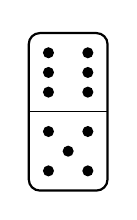
\begin{tikzpicture}
\dominoborder
 \draw (0,0) \fivedots (0,1) \sixdots;
\end{tikzpicture}
\hspace{1em}
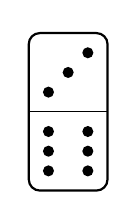
\begin{tikzpicture}
\dominoborder
\draw (0,0) \sixdots (0,1) \threedots;
\end{tikzpicture}
}

How do you know your answer \emph{must} be correct, no matter how you (legally) line up the dominoes?  And most importantly, what does this have to do with Euler paths?

\begin{solution}
  No matter how you arrange the dominoes, the ends will be 1 and 4, with a sum of 5.
  
  Consider the graph consisting of the numbers 1 through 6 as vertices.  Put an edge between two vertices provided there is a domino in the collection above that has those two numbers on it.  We get the following graph.
  
  \centerline{
  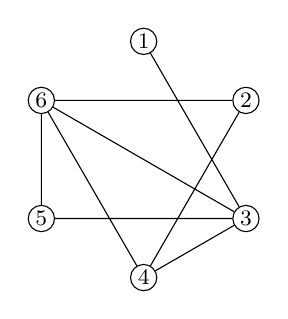
\begin{tikzpicture}
    \foreach \i in {1,...,6}{
    \node[circle, draw, inner sep=1pt] at (150-60*\i: 1.5) (a\i) {\footnotesize \i};
    }
    \draw (a2) -- (a4) (a6) -- (a2) (a1) -- (a3) (a4) -- (a6) (a5) -- (a3) (a4) -- (a3) (a6) -- (a5) (a3) -- (a6);
  \end{tikzpicture}
  }
  
  Every way you lay down all 8 dominoes so that matching numbers touch will correspond to an Euler path through this graph.  Each domino is used once, so each edge is used exactly once; since the numbers must match, we cannot jump between vertices.  Looking at the degrees of vertices in the graph, we see that there are exactly two that are odd: 1 and 4.  Thus these must be the start and stop vertices in the path, so these will be the ends of the row of dominoes.
\end{solution}


	\question[6] Determine whether the following are valid deduction rules.  Your answer should involve a truth table as well as an explanation of what your truth table tells you.
	\begin{multicols}{2}
	\begin{parts}
	  \part ~\\ \begin{tabular}{cc}
	  & $P \imp (Q \vee R)$ \\
	  & $\neg (P \imp Q)$ \\ \hline
	  $\therefore$ & $R$
	  \end{tabular}
	  \columnbreak
	  \part ~\\ \begin{tabular}{cc}
	  & $(P \wedge Q) \imp R$ \\
	  & $\neg P \vee \neg Q$ \\ \hline
	  $\therefore$ & $\neg R$
	  \end{tabular}
	\end{parts}
	\end{multicols}

	\begin{solution}
	  \begin{parts}
	    \part Here is a truth table that includes all the statements:

	        \begin{tabular}{c|c|c||c|c}
	          $P$ & $Q$ & $R$ & $P\imp (Q\vee R)$ & $\neg(P \imp Q)$  \\ \hline
	          T   &  T  &  T  &         T         &      F     \\
	          T   &  T  &  F  &         T         &      F     \\
	          T   &  F  &  T  &         T         &      T     \\
	          T   &  F  &  F  &         F         &      T     \\
	          F   &  T  &  T  &         T         &      F     \\
	          F   &  T  &  F  &         T         &      F     \\
	          F   &  F  &  T  &         T         &      F     \\
	          F   &  F  &  F  &         T         &      F     \\
	        \end{tabular}

	        Notice that there is only one row in which both premises are true (row 3).  In this row, $R$ is also true.  So whenever the premises are true, so is the conclusion.  Thus this is a valid deduction rule.

	        \part Here is the truth table for this proposed rule:

	      \begin{tabular}{c|c|c||c|c|c}
	        $P$ & $Q$ & $R$ & $(P \wedge Q) \imp R$ & $\neg P \vee \neg Q$ & $\neg R$ \\ \hline
	        T   &  T  &  T  &           T            &           F         &   F \\
	        T   &  T  &  F  &           F            &           F         &   T \\
	        T   &  F  &  T  &           T            &           T         &   F \\
	        T   &  F  &  F  &           T            &           T         &   T \\
	        F   &  T  &  T  &           T            &           T         &   F \\
	        F   &  T  &  F  &           T            &           T         &   T \\
	        F   &  F  &  T  &           T            &           T         &   F \\
	        F   &  F  &  F  &           T            &           T         &   T \\
	      \end{tabular}

	      Now look at rows 3. 5 and 7.  In each of these (one would be enough) both premises are true.  However, here the conclusion is false.  Thus this is NOT a valid deduction rule.  In fact, we can see exactly where it goes wrong: If $P$ or $Q$ is false and $R$ is true, we get a counterexample, since $Q$ being false makes both premises true no matter what $R$ is.
	  \end{parts}
	\end{solution}


	\question[9] Consider the statement, ``If a graph is regular or 3-connected, then it is not planar.''  You do not need to know what these terms mean to complete this problem.
	\begin{parts}
		\part Make a truth table for the statement $(R \vee C) \imp \neg P$.
		\part If you believed the statement was \emph{false}, what properties would a counterexample need to possess?  Explain by referencing your truth table.
		\part If the statement were true, what could you conclude about the graph $W_7$, which is definitely planar?  Again, explain using the truth table.
	\end{parts}

\begin{solution}
	\begin{parts}
		\part    \begin{tabular}{c|c|c||c}
						$R$ & $C$ & $P$ & $(R\vee C) \imp \neg P$  \\ \hline
						T   &  T  &  T  &             F     \\
						T   &  T  &  F  &             T     \\
						T   &  F  &  T  &             F     \\
						T   &  F  &  F  &             T     \\
						F   &  T  &  T  &             F     \\
						F   &  T  &  F  &             T     \\
						F   &  F  &  T  &             T     \\
						F   &  F  &  F  &             T     \\
					\end{tabular}

		\part There are three cases in which the statement is false: rows 1, 3 and 5.  So one way to prove this was false would be to find a graph that was regular, 3-connected and planar (row 1).  Or you could find a graph that was triangular, not 3-connected, and planar (row 3) or one that is not regular, is 3-connected and is not planar (row 5).
		\part Here we have a planar graph, so we need to look at rows in which $P$ is true.  We also need the statement to be true.  There is only one row with both these properties: row 7.  And here we see that $R$ and $C$ are both false.  So we would know that $W_7$ is neither regular nor 3-connected.
	\end{parts}
\end{solution}

\question[9] Consider the statement: For any graph, if every vertex has degree 3, then the graph has an even number of vertices.
\begin{parts}
  \part State the converse, contrapositive, and negation of this statement.
  \begin{solution}
    The converse: For any graph, if the graph has an even number of vertices, then every vertex has degree 3.
    
    The contrapositive: For any graph, if the graph has an odd number of vertices, then some vertex does not have degree 3.
    
    The negation: There is a graph for which every vertex has degree 3 but the graph has an odd number of vertices.
  \end{solution}
  \part Give a careful proof of this statement using either a direct proof or a proof by contrapositive.
  \begin{solution}
    We will give a direct proof.  Let $G$ be a graph and assume that every vertex has degree 3.  Let $v$ be the number of vertices and $e$ be the number of edges.  Since every vertex is incident to 3 edges, but each edge is incident to two vertices, we have $e = \frac{3v}{2}$.  This says that $2e = 3v$.  The left hand side is even, so the right hand side must be even as well.  But the only way for a multiple of 3 to be even is for it to be 3 times an even number, so $v$ is even.
  \end{solution}
  \part Give a careful proof of this statement using a proof by contradiction.
  \begin{solution}
    Assume, for the sake of contradiction, that there is some graph $G$ for which every vertex has degree 3 but there are an odd number of vertices.  Say the number of vertices is $v = 2k +1$ for some integer $k$.  We can compute the number of edges by taking $\frac{3v}{2} = \frac{6k+3}{2}$.  But this is not an integer (it is $3k+1 + \frac{1}{2}$), a contradiction.
  \end{solution}
\end{parts}

% \question[6] A \emph{Hamilton path} is a walk that visits every vertex exactly once.  A \emph{Hamilton cycle} is is a Hamilton path that starts and stops at the same vertex (it is okay that the starting/stopping vertex is visited twice, but no other vertex may be).  Consider the following graph:
%
% \begin{center}
% \begin{tikzpicture}[scale=.5]
% \foreach \x in {0, 45, ..., 315}
%   \draw  (\x:2) \v -- (\x+45:2);
% \draw (0,0) \v -- (45:2) (0,0) -- (135:2) (0,0) -- (225:2) (0,0) -- (315:2);
% \draw (-1,0) \v -- (90:2) (-1,0) -- (180:2) (-1,0) -- (270:2);
% \draw (1,0) \v -- (90:2) (1,0) -- (0:2) (1,0) -- (270:2);
% \end{tikzpicture}
% \end{center}
%
% \begin{parts}
% 	\part Find a Hamilton path.  Can your path be extended to a Hamilton cycle?
% 	\part Is the graph bipartite?  If so, how many vertices are in each ``part''?
% 	\part Use your answer to part (b) to prove that the graph has no Hamilton cycle.
% \end{parts}
%
% \begin{solution}
%   \begin{parts}
%     \part One path is shown below:
%
%     \begin{center}
%     \begin{tikzpicture}[scale=.5]
%     \foreach \x in {0, 45, ..., 315}
%       \draw  (\x:2) \v -- (\x+45:2);
%     \draw (0,0) \v -- (45:2) (0,0) -- (135:2) (0,0) -- (225:2) (0,0) -- (315:2);
%     \draw (-1,0) \v -- (90:2) (-1,0) -- (180:2) (-1,0) -- (270:2);
%     \draw (1,0) \v -- (90:2) (1,0) -- (0:2) (1,0) -- (270:2);
%     \draw[ultra thick] (45:2) -- (0,0);
%     \draw[ultra thick] (0,0) -- (135:2);
%     \draw[ultra thick] (135:2) -- (180:2);
%     \draw[ultra thick] (180:2) -- (225:2);
%     \draw[ultra thick] (225:2) -- (270:2);
%     \draw[ultra thick] (270:2) -- (-1,0);
%     \draw[ultra thick] (-1,0) -- (0,2);
%     \draw[ultra thick] (0,2) -- (1,0);
%     \draw[ultra thick] (1,0) -- (2,0);
%     \draw[ultra thick] (2,0) -- (315:2);
%     \end{tikzpicture}
%     \end{center}
%     This path cannot be extended to a cycle (none could be, as seen below).
%     \part Yes, the graph is bipartite. In other words you could 2-color the vertices.  Notice that doing so always gives one side/color 5 vertices and the other 6.
%     \part Notice that any Hamilton path (or cycle) must alternate between sides/colors of the bipartite graph.  To have a path, we must start at one of the vertices on the larger side, but then after visiting all 11 vertices, we will be back on the larger side, so we will not be able to travel to the starting vertex (which is a different vertex on the same side).  In general, this says that if a bipartite graph has a Hamilton cycle, then the two sides of the bipartite graph must have the same size.
%   \end{parts}
% \end{solution}
%
%
% \question[6] Consider the statement: If a graph $G$ is bipartite and one part as at least two more vertices than the other, then $G$ does not have a Hamilton path.
%
% \begin{parts}
% 	\part Write the converse, contrapositive, and negation of the statement.
% 	\part Prove the statement is true.  Clearly identity what style of proof (direct, contrapositive, or contradiction) you use.
% \end{parts}



	\bonusquestion[5] \textbf{Bonus:} You come across four trolls playing bridge.  As you know, all trolls belong to one of two clans: knights, who always tell the truth, or knaves, who always lie.  They declare:
	\begin{itemize}
	\item[] Troll 1: All trolls here see at least one knave.

	\item[] Troll 2: I see at least one troll that sees only knaves.

	\item[] Troll 3: Some trolls are scared of goats.

	\item[] Troll 4: All trolls are scared of goats.
	\end{itemize}

	Are there any trolls that are not scared of goats?  Justify your answer.

	\begin{solution}
	Consider first the statement of Troll 2.  If this were true, then Troll 2 would be a knight.  But the troll he sees that sees only knaves would see him, a knight.  Thus Troll 2 is a knave.  This also means that his statement is false.  In other words, every troll he sees, sees at least one knight.

	Now consider Troll 1's statement.  If this were false, that would mean that there was a troll that saw only knights.  That would have to be Troll 2 (since he is a knave), but Troll 2 sees Troll 1, also a knave.  Thus Troll 1's statement is true, and he is knight.  Also, since his statement is true, everyone sees at least one knave.

	Note that since every troll sees at least one knight (including the knights) and every troll sees at least one knave (including the knaves) there must be exactly two knights and two knaves.

	So among trolls 3 and 4, one is a knight and one is a knave.  The only way this can happen is if Troll 3 is a knight and Troll 4 is a knave (if all trolls are scared of goats, then some are as well).

	In particular, it is false that all trolls are scared of goats, so some strolls are not scared of goats.


	\end{solution}




\end{questions}




\end{document}
